%%
%% 研究報告用スイッチ
%% [techrep]
%%
%% 欧文表記無しのスイッチ(etitle,eabstractは任意)
%% [noauthor]
%%

%\documentclass[submit,techrep]{ipsj}
\documentclass[submit,techrep,noauthor]{ipsj}



\usepackage[dvips]{graphicx}
\usepackage{latexsym}

\def\Underline{\setbox0\hbox\bgroup\let\\\endUnderline}
\def\endUnderline{\vphantom{y}\egroup\smash{\underline{\box0}}\\}
\def\|{\verb|}
%\def\newblock{\hskiip .11em plus .33em minus .07em}

%


%\setcounter{巻数}{59}%vol59=2018
%\setcounter{号数}{10}
%\setcounter{page}{1}


\begin{document}


\title{Code2Vec for C:C言語を対象としたコードの分散表現の獲得手法の提案}

% \etitle{How to Prepare Your Paper for IPSJ SIG Technical Report \\ (version 2018/10/29)}

\affiliate{IPSJ}{九州大学大学院 システム情報科学研究院\\
IPSJ, Faculty of Information Science and Electrical Engineering, Kyushu University}
\paffiliate{JU}{九州大学大学院 システム情報科学府\\
Graduate School of Information Science and Electrical Engineering, Kyushu University}
\paffiliate{F}{富士通九州ネットワークテクノロジーズ(株)\\
Fujitsu Kyushu Network Technologies Limited}

\author{檜枝 琴里}{Kotori Hieda}{JU}[hieda@f.ait.kyushu-u.ac.jp]
\author{久住 憲嗣}{Kenji Hisazumi}{IPSJ}[nel@slrc.kyushu-u.ac.jp]
\author{矢川 博文}{Hirofumi Yagawa}{F}
\author{福田 晃}{Akira Fukuda}{IPSJ}[gakkai.jiro@ipsj.or.jp]

\begin{abstract}
プログラムコードの分散表現を得るための手法としてCode2Vecが存在する.これはプログラムコードの埋め込みベクトルを得るために,メソッド本体などのコード片の機能を表すラベルを予測するタスクで学習するものである.これによりプログラムコードにおいてもコード片の意味を考慮した分散表現を得ることが出来る.Code2VecはJavaやC♯などのオブジェクト指向プログラムを対象としているが,組込みシステム開発ではオブジェクト指向言語ではないC言語を使用していることが多い.そのため,Code2Vecの手法を適用するために,C言語からの特徴量の抽出手法が必要であることや,関数名等の命名方法がオブジェクト指向言語と異なるためラベルの予測が困難といった課題がある.そこで本研究ではCode2Vecの手法をC言語プログラムにも対応可能にすべく,C言語からの特徴量の抽出手法を提案し,関数名等をオブジェクト指向言語と同様のモジュール名と機能名に分解するためのITF-DF手法を提案する.
\end{abstract}


%
%\begin{jkeyword}
%情報処理学会論文誌ジャーナル,\LaTeX,スタイルファイル,べからず集
%\end{jkeyword}
%
%\begin{eabstract}
%This document is a guide to prepare a draft for submitting to IPSJ
%Journal, and the final camera-ready manuscript of a paper to appear in
%IPSJ Journal, using {\LaTeX} and special style files.  Since this
%document itself is produced with the style files, it will help you to
%refer its source file which is distributed with the style files.
%\end{eabstract}
%
%\begin{ekeyword}
%IPSJ Journal, \LaTeX, style files, ``Dos and Dont's'' list
%\end{ekeyword}

\maketitle

%1
\section{序論}
自然言語処理ではWord2Vec\cite{alon2019code2vec}などの意味を考慮した分散表現を得る方法が提案されており様々な応用が展開している.プログラムコードにおいても同様の分散表現を得る手法を使用することにより,ソフトウェア開発を多様な側面から支援することができると考えられるが,手法,応用の両面ともに発展の余地がある.

% code2vecの説明
プログラムコードの分散表現を得る手法としてCode2Vec\cite{alon2019code2vec}が提案されている.Code2Vecとはプログラムコードの分散表現を得るための手法であり,コード片を高次元の実数ベクトルとして表すことで,コード片やそれ同士の関連性を数値的に表現することができる.これによりコードを抽象構文木にして扱うことができるため,コードの終端記号同士間のパスを特徴量として,構造がほぼ同じでも細かい差により機能が変わるものを見分けることが可能となった.このCode2Vecは現状ではJavaやC♯等のオブジェクト指向プログラム言語を対象としている.しかしながら,組込みシステムなどで多く使用されているC言語はオブジェクト指向言語でないため,Code2VecをC言語にそのまま適用できない.具体的には,関数名がモジュール固有名も操作名も含んでいるため,モジュール固有名を重要視してしまうことや,マクロ使用を関数名と混合してしまうなどの課題がある.

% - code2vecの説明を節を分けてした方が良いと思います。code2vecの論文を見ながら概要を書いてもらうと良いと思いますが、特徴としては、従来はコードの構成要素のみを特徴量としていたのが、コードの終端記号と終端記号の間のパスを特徴量とすることで、コードの構造はほぼ同じだけれども細かい違いにより機能が変わるもの(配列の中からアイテムを取得する、配列の中にアイテムが存在するか?等)を見分けることが可能になったところかなと思います。
そこで本研究ではこの課題を解決すべく,TF-IDF手法 (…) を関数名に適用する.TF-IDF手法とはある文書の中での出現頻度は低いが様々な文書を通して見ると出現頻度が高い単語の重要度が高くなるようにするものである.これによりモジュール固有名と操作名とを選別し,操作名のみを学習する手法を提案する.これにより,一つのプログラムコード内で頻繁に出てくる,それ特有でしかないモジュール固有名の重要度を下げ,広く一般的に使用される操作名の重要度を上げることを狙う.重要な操作名に重みがついた状態で学習することにより,関数名推定の精度向上を図る.

具体的には,C言語で記述されたプログラムコードをいくつか用意し,ITF-DF手法を用いて重み付けをした関数名を学習する.学習したコード片に基づきC言語にも対応させたCode2Vecを用いることで,コード片をベクトルとし,関連のあるコード片同士を紐付ける.評価の方法として,評価をするためのプログラムコードを用意し,その中の関数名と,関数名推定を行った結果とを照らし合わせ,元の関数名との適合率を表す.

\begin{table*}[t]
 \centering
 \caption{ITF-DF手法を用いた推定結果}
 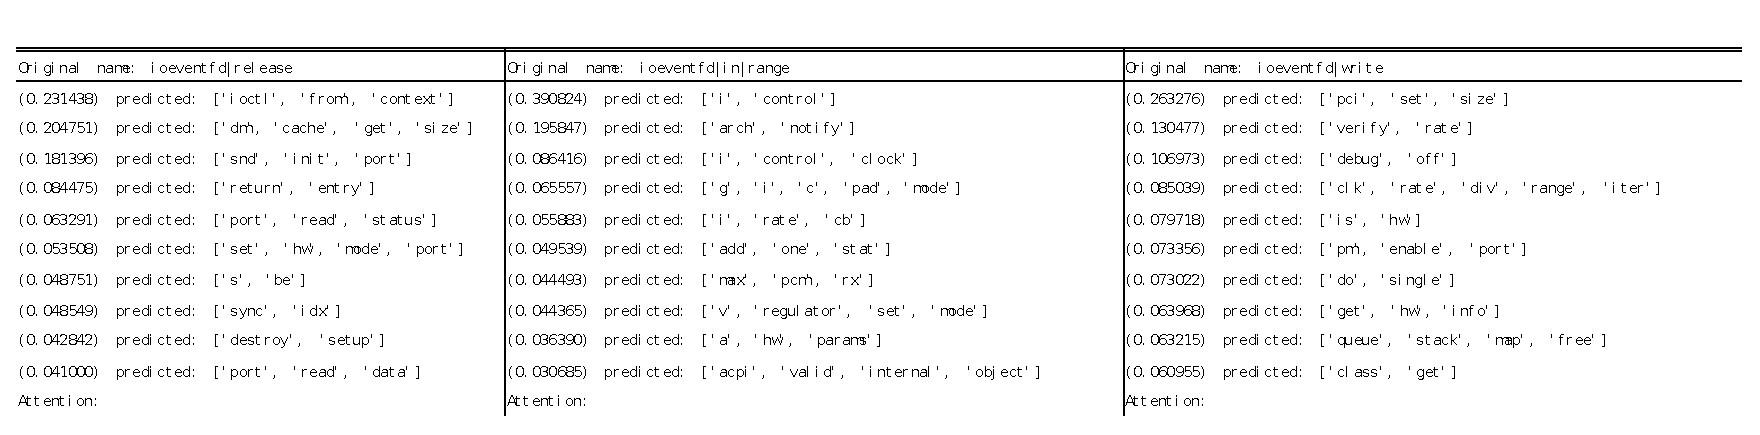
\includegraphics[width=1.0\hsize]{image/result.eps} 
 \label{table1} 
\end{table*}


%2
\section{解析手法}

% LLVMとclangの説明
本研究ではC言語で書かれているプログラムコードをいくつか用意し,その中の関数名を,Code2Vecを用いて分散表現し,モジュール名と機能名に分類した.Code2VecはC言語のような非オブジェクト指向言語を対象としていないため,コンパイラフロントエンドのClangとバックエンドのLLVMを用いてC言語にもCode2Vecを応用できるようにした.LLVMは,中間言語を介して対象のアーキテクチャに最適なマシン語へ変換することができるため,多様なプラットフォームで最適なマシン語へ変換することができる.ClangはLLVM上で動作することを意図し設計されている.これらのコンパイラは,統合開発環境(IDE)のGUIと密接に連携し開発できるようにしてあり,様々な環境でのクロスプラットフォーム開発を容易にし,C言語をターゲットとして設計されているため,本研究に用いた.

% - 解析手法の節では、評価に関する記述はすべて除きます。代わりに特徴量の抽出手順を丁寧に説明します。また、clang/llvmなどの可能な限りプラットフォームなどの実装依存の説明と、アルゴリズムの説明を分離します。そして、まず一般性の高いアルゴリズムから説明します。できれば両者は小節を分けた方が良いでしょうね。
モジュール名と機能名に分類した関数名を,ITF-DF手法により{log (文書Aにおける単語Xの出現頻度) / (文書Aにおける全単語の出現頻度の和)} * {(全文書数) / (単語Xを含む文書数)} と計算し,ある文書の中での出現頻度は低いが様々な文書を通して見ると出現頻度が高い単語の重要度が高くなるように重み付けをした.さらにモジュール名と機能名に分類し重み付けをした関数名を,関数の内容と紐づけて学習した.これを辞書として用意し,関数の内容からその関数名として適切だと思われるものを,辞書から選び提案する.
%ITF-DF手法を使って関数名などをモジュール名と機能名に分解して学習する.学習したらテストデータでうまくいくか試してみる.



%3
\section{結果}
学習したデータを基に,テスト用に用意した関数の内容をシステムに読み込ませ,その関数名を推定させる.元の関数名との適合率を評価の基準として表す.
表~\ref{table1} は関数名推定結果の一部である.推定の結果,テストデータとして用意していたC言語プログラムコードにあらかじめ設定されていた関数名と同じ関数名を推定することができた.しかしその精度は必ずしも高いとは言えず,全く別の関数名を推定する場合もあった.
% 間違えてるのもあるけどなんとなくうまくいった.
% 〜〜(推定結果の図か表)〜〜

%4
\section{結論}
今回,我々はLLVMとClangを用いてCode2VecをC言語に対応可能な状態にした.またそれを適用する事でC言語の関数名をモジュール名と機能名に分類し,ITF-DF手法により重み付けしたものを機械学習することで関数名推定の精度を向上を試みた.結果,ITF-DF手法を用いることで,汎用的に用いられれいるモジュール名を抜き出すことが可能となり,関数名推定の精度が向上することがわかった.\\
今後の予定として,より多くのテストデータを用いての詳細な評価を試みる.また現在よりも更に精度が向上するITF-DF手法の計算方法を模索する.それを再度評価することで,C言語特有の拡張が可能となることを期待する.


% うまくいった.ラッキー.


% 謝辞
% \begin{acknowledgment}
% A4横型に対するガイドを基に,本稿を作成した.
% クラスファイルの作成においては,
% 京都大学の中島 浩氏にさまざまなご教示を頂き,
% さらにBiB\TeX 関連ファイルの利用についても快諾頂いたことを深謝する.
% また,A4横型に対するガイドを作成された当時の編集委員会の担当者に深謝する.
% \end{acknowledgment}


\bibliographystyle{ipsjunsrt}
\bibliography{bibsample}

% \begin{thebibliography}{10}


% \bibitem{okumura}
% 奥村晴彦:改訂第5版\LaTeXe 美文書作成入門,
% 技術評論社(2010).

% \bibitem{companion}
% Goossens, M., Mittelbach, F. and Samarin, A.:
% {\it The LaTeX Companion},
% Addison Wesley, Reading, Massachusetts (1993).

% \bibitem{book1}
% 木下是雄:
% 理科系の作文技術,
% 中公新書(1981).

% \bibitem{book2}
% Strunk W. J. and White E.B.:
% {\it The Elements of Style, Forth Edition},
% Longman (2000).

% \bibitem{book3}
% Blake G. and Bly R.W.:
% {\it The Elements of Technical Writing},
% Longman (1993).

% \bibitem{book4}
% Higham N.J.:
% {\it Handbook of Writing for the Mathematical Sciences},
% SIAM (1998).

% \bibitem{webpage1}
% 情報処理学会論文誌ジャーナル編集委員会:
% 投稿者マニュアル(online),
% \urlj{http://www.ipsj.or.jp/journal /submit/manual/j\_manual.html}
% (2007.04.05).

% \bibitem{webpage2}
% 情報処理学会論文誌ジャーナル編集委員会:
% べからず集(online),
% \urlj{http://www.ipsj.or.jp/journal/manual /bekarazu.html}
% (2011.09.15).

% \end{thebibliography}




\end{document}
